\section{Implementation}
\label{sec:implementation}

This Section will detail the implementation of the specification described in Section \ref{sec:specification}, highlighting the differences between what was previously specified and the final implementation.

Similar to Section \ref{sec:specification}, this section will first present the nodes that are common to all trees and their representation, then each subtree of the strategy tree will be briefly introduced and any implementation details will be elucidated. All images of nodes and trees shown in this section were taken using the \textit{Groot 2} interface (see Subsubsection \ref{subsubsec:groot}).

\subsection{Common Nodes}
\label{subsec:common_nodes_impl}

The common nodes presented in this section are mostly very similar to the nodes presented in the Subsection \ref{subsec:common_nodes_spec}, changing just their representation. However, due to the implementation of the \textit{BehaviorTree.CPP} library, some of the nodes changed drastically and these changes will be clarified.

\subsubsection{Root Node}

The root node is represented as shown in Figure \ref{fig:root_node_impl}.

\begin{figure}[!h]
    \centering
    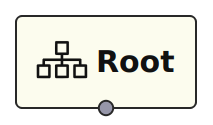
\includegraphics[width=0.15\linewidth]{images/implementation/RootNode.png}
    \caption{Root node in \textit{Groot}}
    \label{fig:root_node_impl}
\end{figure}

\subsubsection{Control Nodes}

In contrast to the representation of control nodes discussed in Subsubsection \ref{subsubsec:control_nodes_spec}, the default behavior of a control node in the \textit{BehaviorTree.CPP} library is to be non-reactive. Therefore,  as can be seen in Figure \ref{fig:control_nodes_impl}, nodes that deviate from this default behavior are denoted as reactive nodes, rather than marking the non-reactive nodes differently.

\begin{figure}[!h]
    \centering
    \begin{subfigure}[b]{.32\linewidth}
        \centering
        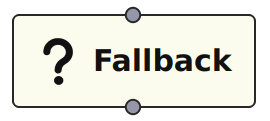
\includegraphics[width=0.52\linewidth]{images/implementation/FallbackNode.png}
        \caption{Non-reactive fallback}
    \end{subfigure}
    \hfill
    \begin{subfigure}[b]{.32\linewidth}
        \centering
        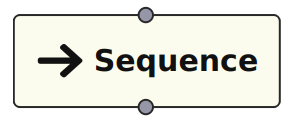
\includegraphics[width=0.57\linewidth]{images/implementation/SequenceNode.png}
        \caption{Non-reactive sequence}
    \end{subfigure}
    \hfill
    \begin{subfigure}[b]{.32\linewidth}
        \centering
        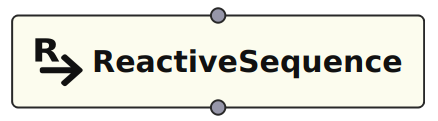
\includegraphics[width=0.8\linewidth]{images/implementation/ReactiveSequenceNode.png}
        \caption{Reactive sequence}
    \end{subfigure}
    \caption{Used control nodes representations in \textit{Groot}}
    \label{fig:control_nodes_impl}
\end{figure}

\subsubsection{Action Nodes}

The implementation of the common action nodes, in Figure \ref{fig:common_action_node_impl}, is very similar to the specification presented in Subsubsection \ref{subsubsec:common_action_nodes_spec}, the \texttt{Always Success} node is precisely the same and the node that sets a variable in the blackboard is a little bit different. In the tree specification, all blackboard variables were represented as strings or booleans, however, in the implementation, some of those variables were created as integer variables instead, therefore, two nodes that store variables in the blackboard were used, one that stores strings and another that stores integers. These two nodes have the same syntax, in the node, the \texttt{value} field receives the value to be stored in the blackboard and the \texttt{output\_key} receives the name of the variable where the value will be stored. One thing important to note is that the node in Figure \ref{fig:set_blackboard_string_impl} is a built-in node of the library, while the node in Figure \ref{fig:set_blackboard_int_impl} is a custom node made inspired by the node from the library.

\begin{figure}[!h]
    \centering
    \begin{subfigure}[b]{.32\linewidth}
        \centering
        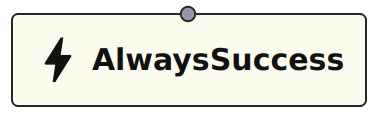
\includegraphics[width=0.7\linewidth]{images/implementation/AlwaysSuccessNode.png}
        \caption{Always success}
    \end{subfigure}
    \hfill
    \begin{subfigure}[b]{.32\linewidth}
        \centering
        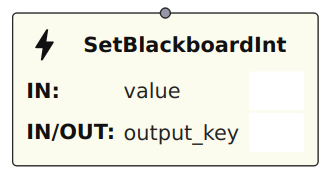
\includegraphics[width=0.85\linewidth]{images/implementation/SetBlackboardIntNode.png}
        \caption{Set Blackboard Int}
        \label{fig:set_blackboard_int_impl}
    \end{subfigure}
    \hfill
    \begin{subfigure}[b]{.32\linewidth}
        \centering
        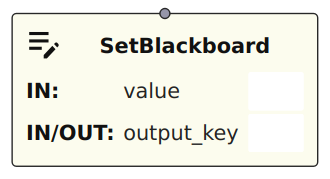
\includegraphics[width=0.85\linewidth]{images/implementation/SetBlackboardStringNode.png}
        \caption{Set Blackboard String}
        \label{fig:set_blackboard_string_impl}
    \end{subfigure}
    \caption{Common used action nodes representation in \textit{Groot}}
    \label{fig:common_action_node_impl}
\end{figure}

\subsubsection{Condition Nodes}

In contrast to the tree specification, the common condition node specified in Subsubsection \ref{subsubsec:common_condition_nodes_spec} is no longer used in the tree implementation, a decorator is used instead, as it will be explained in the next subsubsection.

\subsubsection{Decorator Nodes}

The tree specification was created using condition nodes that verify whether the content of a variable in the blackboard is equal to a specified value and return success or failure depending on the result. However, the \textit{BehaviorTree.CPP} library does not provide a built-in condition node with the described behavior, instead, the library offers decorators that can be used for the same purpose. 

Two decorators from the library were used to substitute the condition nodes, the \texttt{Blackboard Check Int}, in Figure \ref{fig:blackboard_check_int_impl}, and the \texttt{Blackboard Check String}, in Figure \ref{fig:blackboard_check_string_impl}. Both these nodes are very similar, they compare a value A with a value B, if both values are equal, this node will return the same status of its child otherwise it will return the value specified in the "return\_on\_mismatch" field. The difference between these two decorators is just the variable type that they accept, as the first accepts integers and the second accepts strings. One important thing to note is how these nodes actually access variables' values in the blackboard. This is accomplished by specifying the variable's name using the syntax \texttt{\{variable\_name\}}. By employing this syntax, the variable's value will be substituted during the comparison process, so it can be compared to the value in the other field. 

\begin{figure}[!h]
    \centering
    \begin{subfigure}[b]{.49\linewidth}
        \centering
        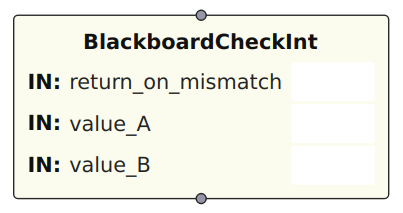
\includegraphics[width=0.65\linewidth]{images/implementation/BlackboardCheckIntNode.png}
        \caption{Blackboard Check Int}
        \label{fig:blackboard_check_int_impl}
    \end{subfigure}
    \hfill
    \begin{subfigure}[b]{.49\linewidth}
        \centering
        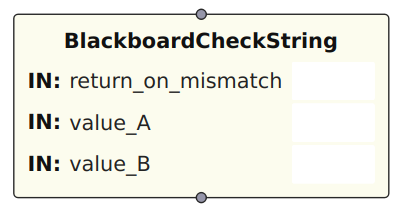
\includegraphics[width=0.65\linewidth]{images/implementation/BlackboardCheckStringNode.png}
        \caption{Blackboard Check String}
        \label{fig:blackboard_check_string_impl}
    \end{subfigure}
    \caption{Blackboard Check decorator nodes representation in \textit{Groot}}
    \label{fig:common_decorator_nodes_impl}
\end{figure}

Regarding the use of these decorators, as it is not possible to simply replace a condition node with a decorator, it was necessary to make changes to the structure of the tree specification where the condition nodes which check the blackboard were used. To implement these modifications, an analysis of the structure which utilizes the \texttt{Blackboard Check} as a condition node was conducted, leading to the development of two alternative approaches using the \texttt{Blackboard Check} decorator implementation of the library. 

Considering the tree specification, all the use cases of the \texttt{Blackboard Check} as a condition node can be abstracted as the two structures in Figure \ref{fig:blackboard_check_eq_condition_node}. The first structure, Figure \ref{fig:blackboard_check_eq_condition_node_fall}, represents the cases where the condition node is used as the first child of a non-reactive fallback, whereas the second structure, Figure \ref{fig:blackboard_check_eq_condition_node_seq}, represents the cases where the parent node of the condition node is a non-reactive sequence instead.

\begin{figure}[!h]
    \centering
    \begin{subfigure}[b]{.49\linewidth}
        \centering
        \scalebox{0.74} {
            \begin{forest}
                [\root, controlflow
                    [\fallback, controlflow
                        [{Blackboard Check \\ variable == value}, condition]
                        [{Conditional Action}, action]
                    ]
                ]
            \end{forest}
        }
        \caption{\texttt{Blackboard Check} as a condition node in a fallback}
        \label{fig:blackboard_check_eq_condition_node_fall}
    \end{subfigure}
    \hfill
    \begin{subfigure}[b]{.49\linewidth}
        \centering
        \scalebox{0.74} {
            \begin{forest}
                [\root, controlflow
                    [\sequence, controlflow
                        [{Blackboard Check \\ variable == value}, condition]
                        [{Conditional Action}, action]
                    ]
                ]
            \end{forest}
        }
        \caption{\texttt{Blackboard Check} as a condition node in a sequence}
        \label{fig:blackboard_check_eq_condition_node_seq}
    \end{subfigure}
    \caption{Tree structures abstraction when using the \texttt{Blackboard Check} as a condition node}
    \label{fig:blackboard_check_eq_condition_node}
\end{figure}

The first alternative to use the described decorator instead of the condition node can be seen in Figure \ref{fig:blackboard_check_eq_action_in_sequence}, in which the condition node is replaced by a decorator configured to return failure when there is a mismatch in the comparison and to return its child status when there is a match, which will always be a success, mimicking the behavior of the condition node. This approach can be used as an alternative to both cases presented in Figure \ref{fig:blackboard_check_eq_condition_node}.

The second alternative, illustrated in Figure \ref{fig:blackboard_check_eq_action_as_child}, is a less verbose approach, using the decorator in a more standard manner, instead of using it to mimic the behavior of a condition node. As this solution requires fewer nodes than the first alternative, it presents itself as a better option. However, this approach cannot be used for both cases depicted in Figure \ref{fig:blackboard_check_eq_condition_node}, as its behavior only corresponds to the behavior of the structure in Figure \ref{fig:blackboard_check_eq_condition_node_seq}.

Therefore, the tree implementation, which will be presented in the next subsections, was structured in a way to adapt the tree specification using these alternatives. In the tree parts where the structure depicted in Figure \ref{fig:blackboard_check_eq_condition_node_fall} is utilized, the alternative approach illustrated in Figure \ref{fig:blackboard_check_eq_action_in_sequence} was employed to simulate a condition node. Conversely, in the parts where the structure depicted in Figure \ref{fig:blackboard_check_eq_condition_node_seq} is present, the alternative approach from Figure \ref{fig:blackboard_check_eq_action_as_child} was utilized.

\begin{figure}[!h]
    \centering
    \begin{subfigure}[b]{.49\linewidth}
        \centering
        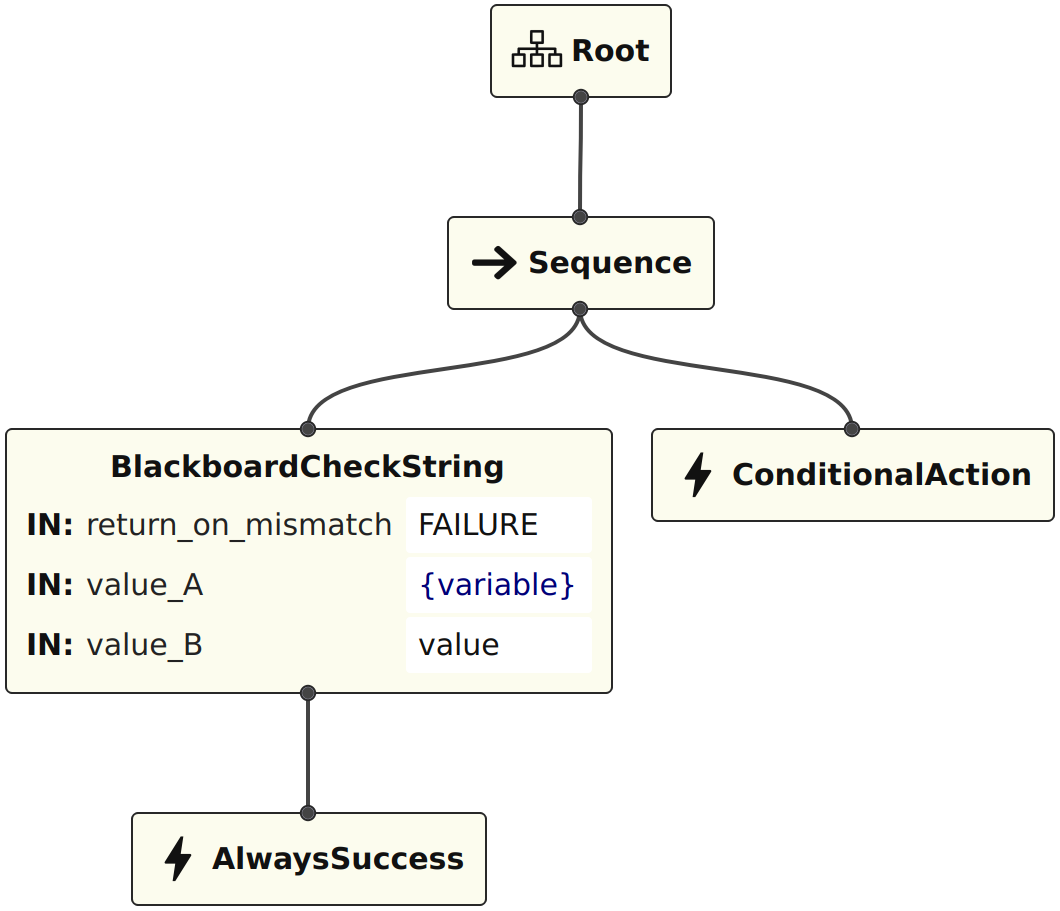
\includegraphics[width=0.85\linewidth]{images/implementation/BlackboardCheck - Equivalence 1.png}
        \caption{\texttt{Blackboard Check} as a decorator with conditional action in sequence}
        \label{fig:blackboard_check_eq_action_in_sequence}
    \end{subfigure}
    \hfill
    \begin{subfigure}[b]{.49\linewidth}
        \centering
        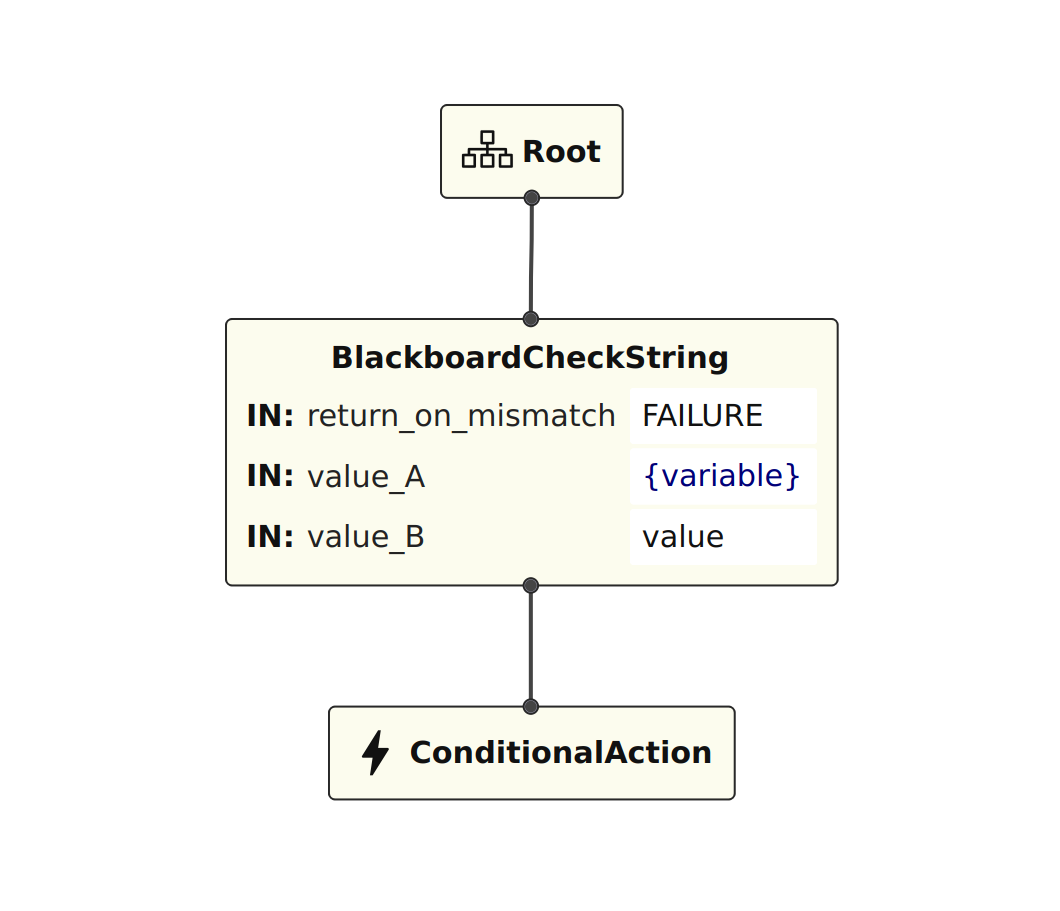
\includegraphics[width=0.85\linewidth]{images/implementation/BlackboardCheck - Equivalence 2.png}
        \caption{\texttt{Blackboard Check} as a decorator with conditional action as child}
        \label{fig:blackboard_check_eq_action_as_child}
    \end{subfigure}
    \caption{Equivalent tree structures when using the \texttt{Blackboard Check} node}
    \label{fig:blackboard_check_equivalences}
\end{figure}

\subsubsection{Subtrees}

The representation of a subtree in the \textit{BehaviorTree.CPP} library, shown in Figure \ref{fig:subtrees_impl}, is very similar to the subtree specification described in the Subsubsection \ref{subsubsec:subtrees_spec}. The only notable difference between the two is that the library's implementation has an attribute called \texttt{\_\_shared\_blackboard}, which is used to specify whether the subtree will have its own blackboard or whether the tree which includes this subtree will share its blackboard with the subtree. In addition, the representation of a subtree node in \textit{Groot} also has a button that can be used to expand the subtree node and view the entire subtree.

\begin{figure}[!h]
    \centering
    \begin{subfigure}[b]{.49\linewidth}
        \centering
        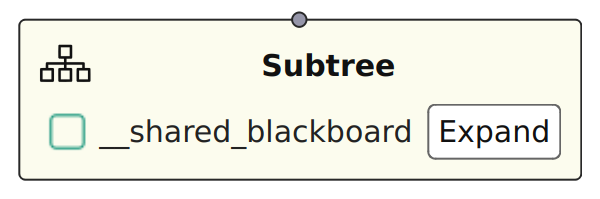
\includegraphics[width=0.6\linewidth]{images/implementation/SubtreeNode - Not Shared BB.png}
        \caption{Subtree without shared blackboard}
    \end{subfigure}
    \hfill
    \begin{subfigure}[b]{.49\linewidth}
        \centering
        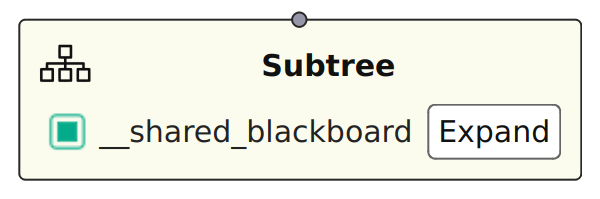
\includegraphics[width=0.6\linewidth]{images/implementation/SubtreeNode - Shared BB.png}
        \caption{Subtree with shared blackboard}
    \end{subfigure}
    \caption{Subtree node representation in \textit{Groot}}
    \label{fig:subtrees_impl}
\end{figure}

% \subsection{Behaviors Controller Tree}

% The \textit{Behaviors Controller} tree implementation is basically the same as its specification, being the only notable difference the fact that it is now made explicit in the trees that they have a shared blackboard, by setting the \texttt{\_\_shared\_blackboard} to true.

% \begin{figure}[!h]
%     \centering
%     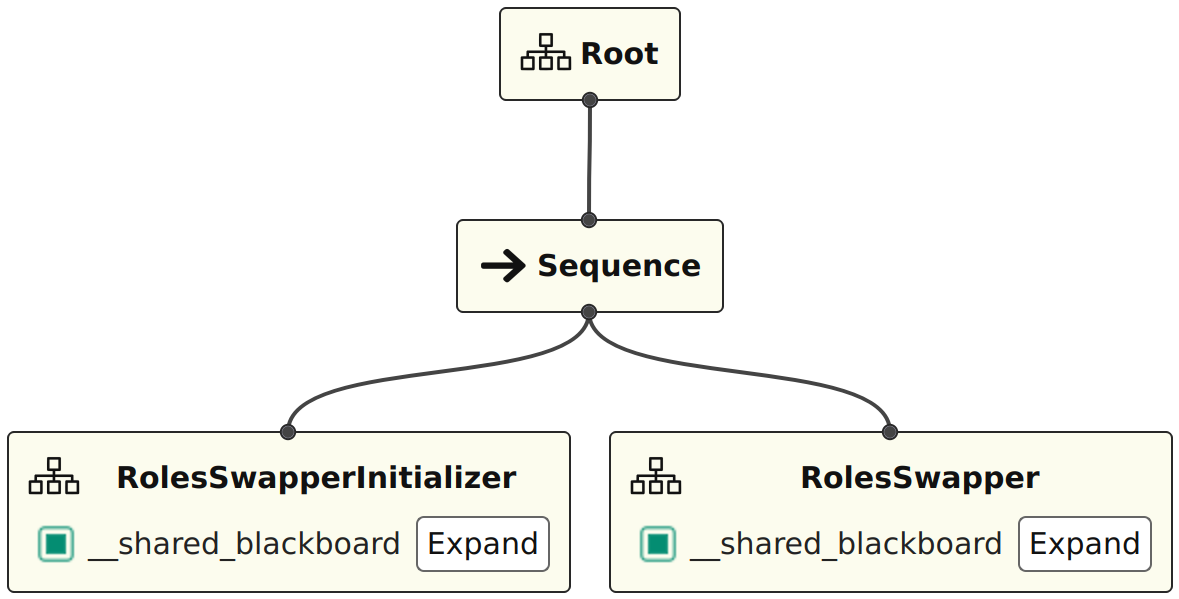
\includegraphics[width=0.7\linewidth]{images/implementation/BehaviorsController.png}
%     \caption{Base structure implementation of the Coach’s Behavior Tree}
%     \label{fig:behaviors_controller_bt_impl}
% \end{figure}

% \subsection{Roles Swapper Initializer}

% In the implementation of the \texttt{Roles Swapper Initializer}, modifications were made to the tree specification, taking into account the information provided about the common nodes in Subsection \ref{subsubsec:common_action_nodes_spec}. The resulting implementation is depicted in Figure \ref{fig:roles_swapper_initializer_impl}. It is important to note that there is one implementation detail in this tree that deviates from its original specification, which is the data types of the variables stored in the blackboard.

% \begin{figure}[!h]
%     \centering
%     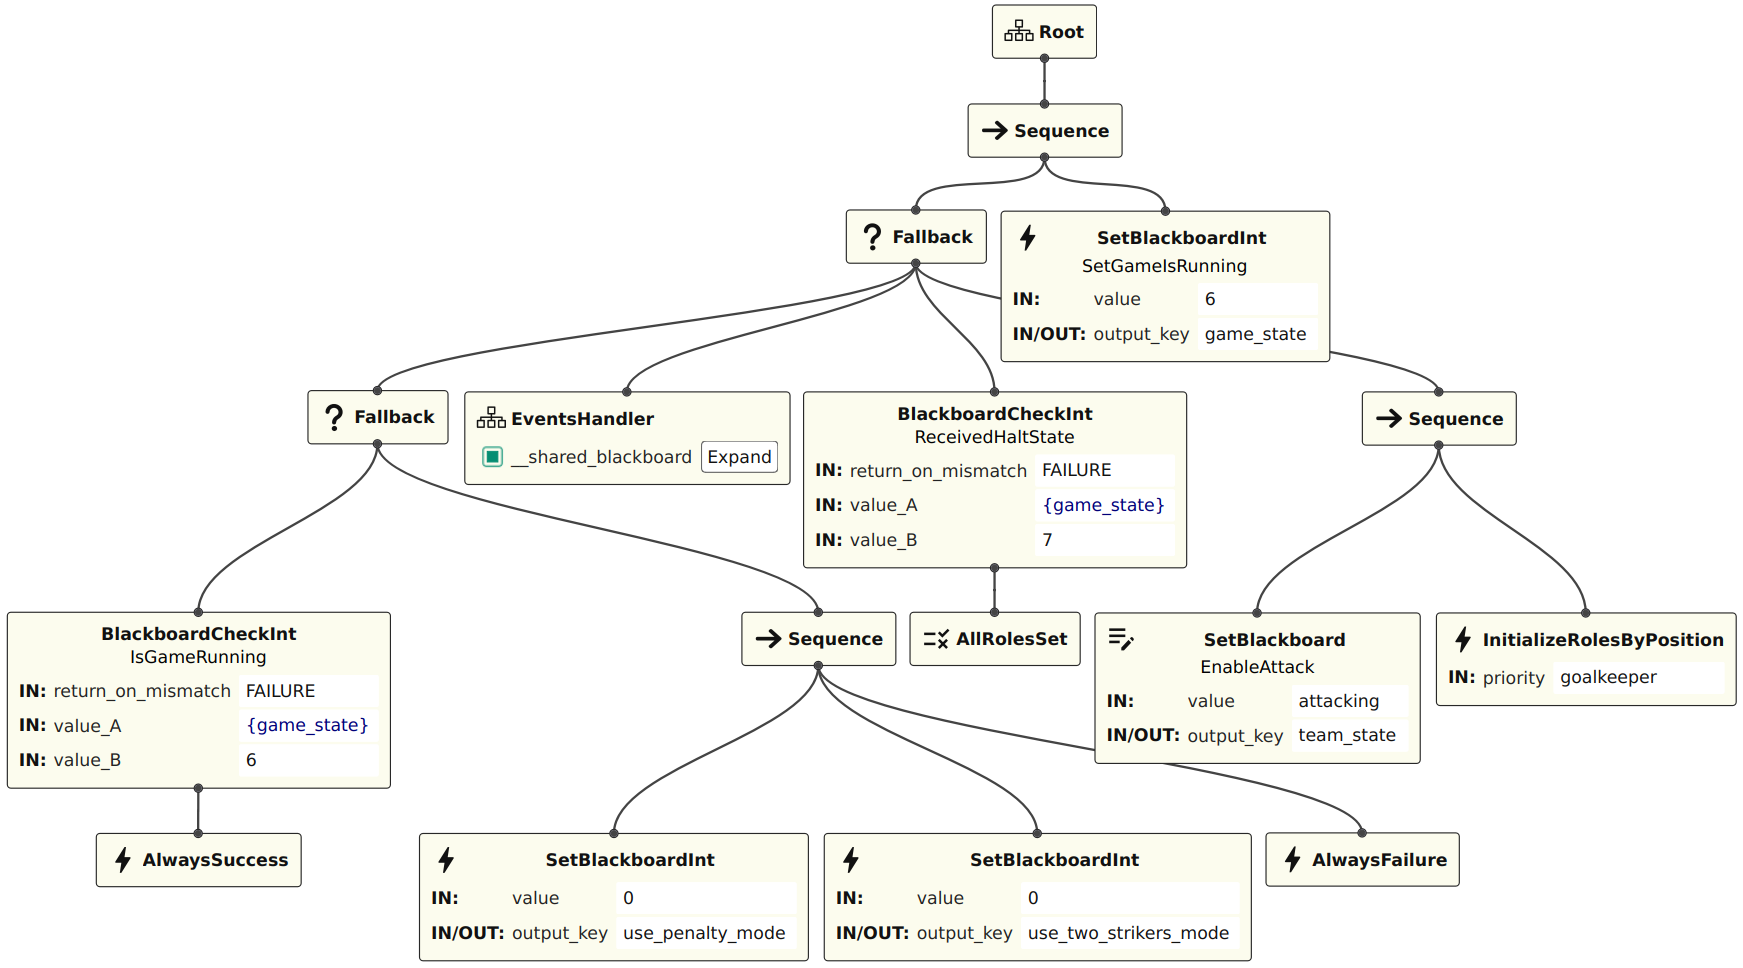
\includegraphics[width=1.0\linewidth]{images/implementation/RolesSwapperInitializer.png}
%     \caption{Roles Swapper Initializer subtree specification}
%     \label{fig:roles_swapper_initializer_impl}
% \end{figure}

% In this tree and its subtrees, six blackboard variables are manipulated, which are the \texttt{game\_state}, the \texttt{game\_state\_team}, the \texttt{game\_state\_side}, the \texttt{use\_penalty\_mode}, the \texttt{use\_two\_strikers\_mode} and the \texttt{team\_state}. 

% In the tree specification, the \texttt{game\_state}, the \texttt{game\_state\_team} and the \texttt{game\_state\_side} variables were all presented as strings for simplifications reasons, however, none of the real messages received from the \textit{VSSReferee} use strings to represent the data, just integers (see Tables \ref{tab:referee_events_ids}, \ref{tab:target_team_event_codification} and \ref{tab:field_side_event_codification}), therefore, the type of these variables in the blackboard was changed to integer. 

% The \texttt{use\_penalty\_mode} and the \texttt{use\_two\_strikers\_mode} variables were previously declared as booleans, nevertheless, to take advantage of the formerly developed \texttt{Set Blackboard Int} node, their data types were changed to integers as well, being \texttt{0} equivalent to \texttt{False} and \texttt{1} to \texttt{True}. 

% The last variable, the \texttt{game\_state}, did not have its data type changed, it remained as a string for reasons of simplification and easier understanding of the tree.

% \begin{table}[!htbp]
%     \centering
%     \begin{tabular}{c c}
%         \toprule
%         Event Name   & Value \\ 
%         \midrule
%         Free Kick    & 0     \\ 
%         Penalty Kick & 1     \\ 
%         Goal Kick    & 2     \\ 
%         Free Ball    & 3     \\ 
%         Kickoff      & 4     \\ 
%         Stop         & 5     \\ 
%         Game On      & 6     \\ 
%         Halt         & 7     \\ 
%         \bottomrule
%     \end{tabular}
%     \caption{Integer identifications of the events sent by the \textit{VSSReferee}, see \cite{VSSProto}}
%     \label{tab:referee_events_ids}
% \end{table}

% \begin{table}[!htbp]
%     \centering
%     \begin{tabular}{c c}
%         \toprule
%         Target Team & Value \\ 
%         \midrule
%         Friends     & 0     \\ 
%         Foes        & 1     \\ 
%         \bottomrule
%     \end{tabular}
%     \caption{Codification of the target team of the event received from the \textit{VSSReferee}, using the event and the team color}
%     \label{tab:target_team_event_codification}
% \end{table}

% \begin{table}[!htbp]
%     \centering
%     \begin{tabular}{c c}
%         \toprule
%         Side of field & Value \\ 
%         \midrule
%         Friends' side & 0     \\ 
%         Foes' side    & 1     \\ 
%         \bottomrule
%     \end{tabular}
%     \caption{Codification of the side of the field in which the event received from the \textit{VSSReferee} occurred, using the event and the team color}
%     \label{tab:field_side_event_codification}
% \end{table}

% \subsection{Events Handler and its subtrees}

% The \texttt{Events Handler} subtree has the same structure as its specification, the only difference from its specification is that it defines the \texttt{\_\_shared\_blackboard} attributes of its subtrees. The implementation can be seen in Figure \ref{fig:events_handler_impl}.

% \begin{figure}[!h]
%     \centering
%     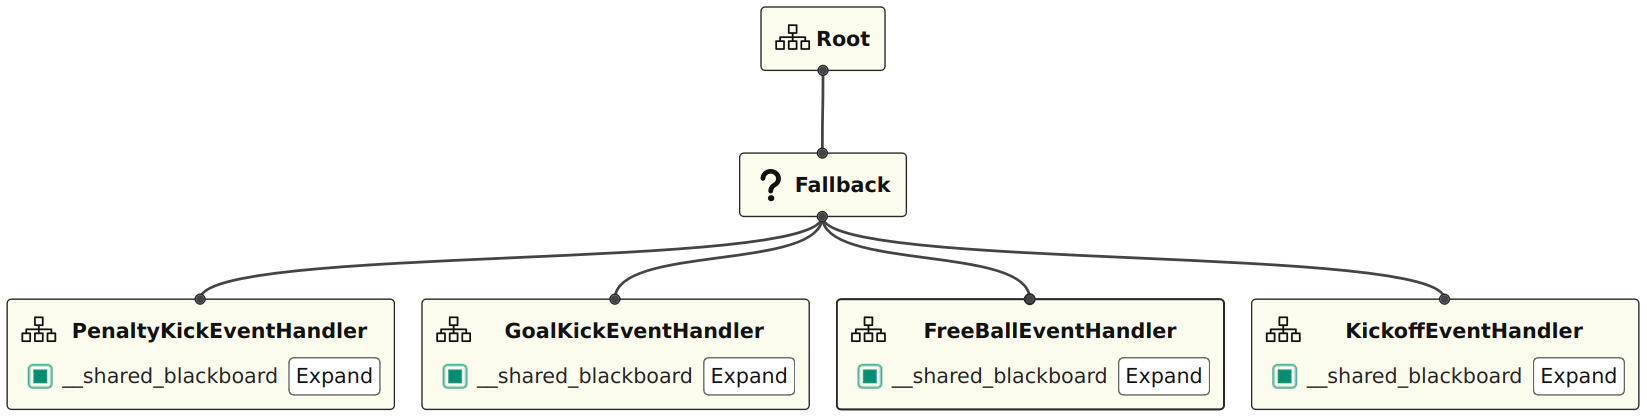
\includegraphics[width=1.0\linewidth]{images/implementation/EventsHandler.png}
%     \caption{Events Handler subtree implementation}
%     \label{fig:events_handler_impl}
% \end{figure}

% Considering the changes presented in Subsection \ref{subsec:common_nodes_impl} and the changes to the data types of the variables on the blackboard, the implementations of all subtrees of the \texttt{Events Handler} subtree are analogous to their specifications. The implementations of the four subtrees are represented in Figures \ref{fig:penalty_kick_event_handler_impl}, \ref{fig:goal_kick_event_handler_impl}, \ref{fig:free_ball_event_handler_impl} and \ref{fig:kickoff_event_handler_impl}.

% One simple implementation detail that deserves attention is the presence of parameters in the \texttt{Set Penalty Mode} node in the \texttt{Penalty Kick Event Handler}. These parameters were added to the node so it could be more generic, instead of having those values hardcoded to the node's code.

% \begin{figure}[!h]
%     \centering
%     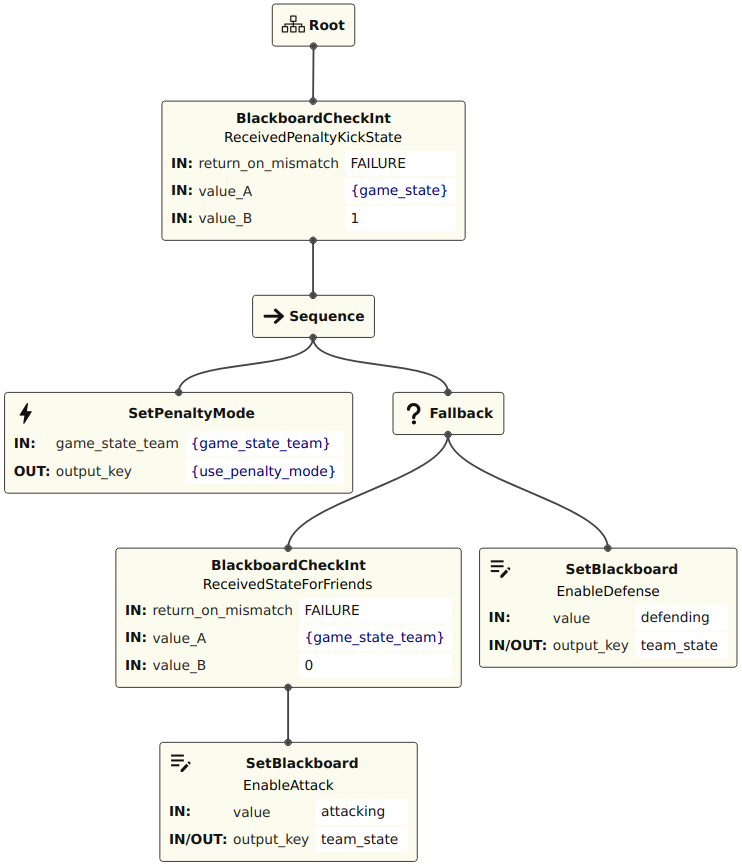
\includegraphics[width=0.7\linewidth]{images/implementation/PenaltyKickEventHandler.png}
%     \caption{Penalty Kick Event Handler subtree implementation}
%     \label{fig:penalty_kick_event_handler_impl}
% \end{figure}

% \begin{figure}[!h]
%     \centering
%     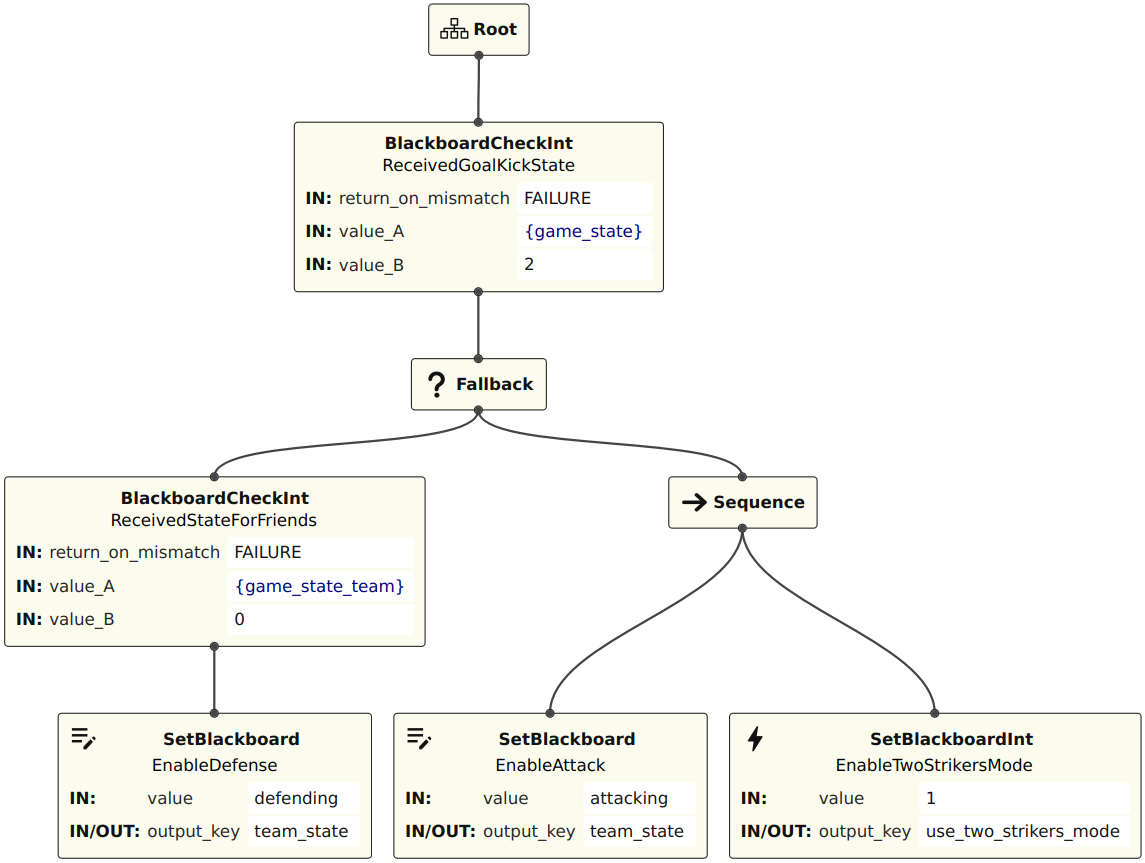
\includegraphics[width=0.9\linewidth]{images/implementation/GoalKickEventHandler.png}
%     \caption{Goal Kick Event Handler subtree implementation}
%     \label{fig:goal_kick_event_handler_impl}
% \end{figure}

% \begin{figure}[!h]
%     \centering
%     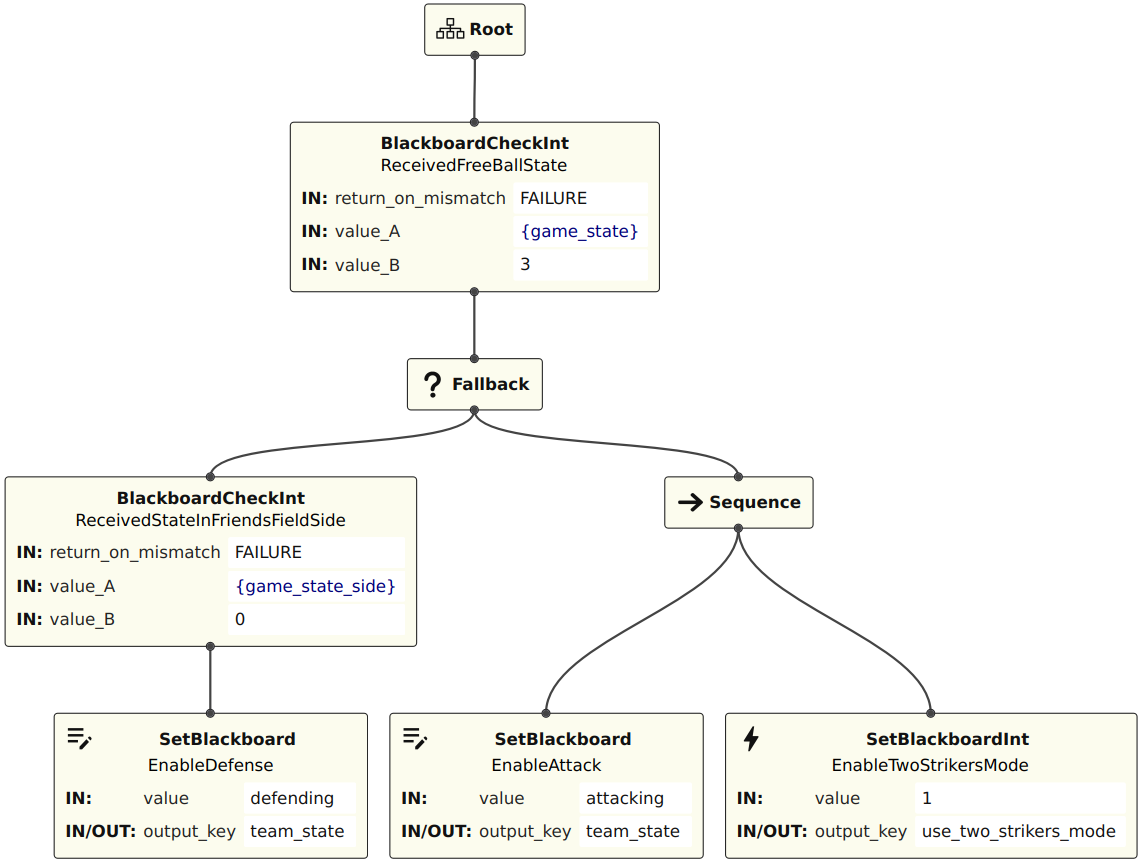
\includegraphics[width=0.9\linewidth]{images/implementation/FreeBallEventHandler.png}
%     \caption{Free Ball Event Handler subtree implementation}
%     \label{fig:free_ball_event_handler_impl}
% \end{figure}

% \begin{figure}[!h]
%     \centering
%     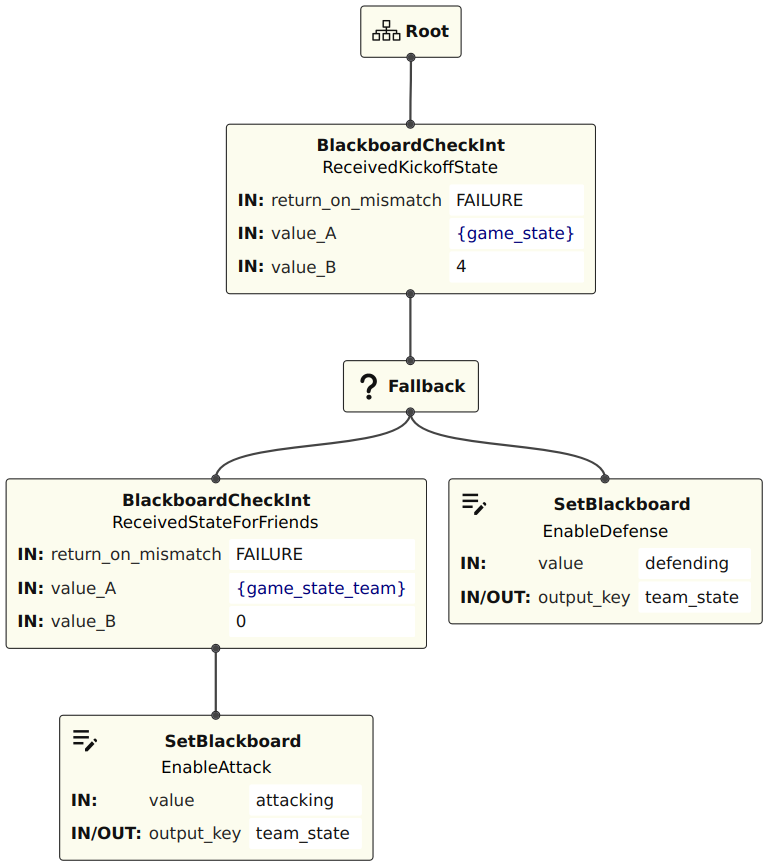
\includegraphics[width=0.65\linewidth]{images/implementation/KickoffEventHandler.png}
%     \caption{Kickoff Event Handler subtree implementation}
%     \label{fig:kickoff_event_handler_impl}
% \end{figure}

% \subsection{Roles Swapper}

% Taking into account the insights discussed in Subsection \ref{subsec:common_nodes_impl}, the implementation of \texttt{Roles Swapper} adheres closely to its specification, as depicted in Figure \ref{fig:roles_swapper_impl}.

% \begin{figure}[!h]
%     \centering
%     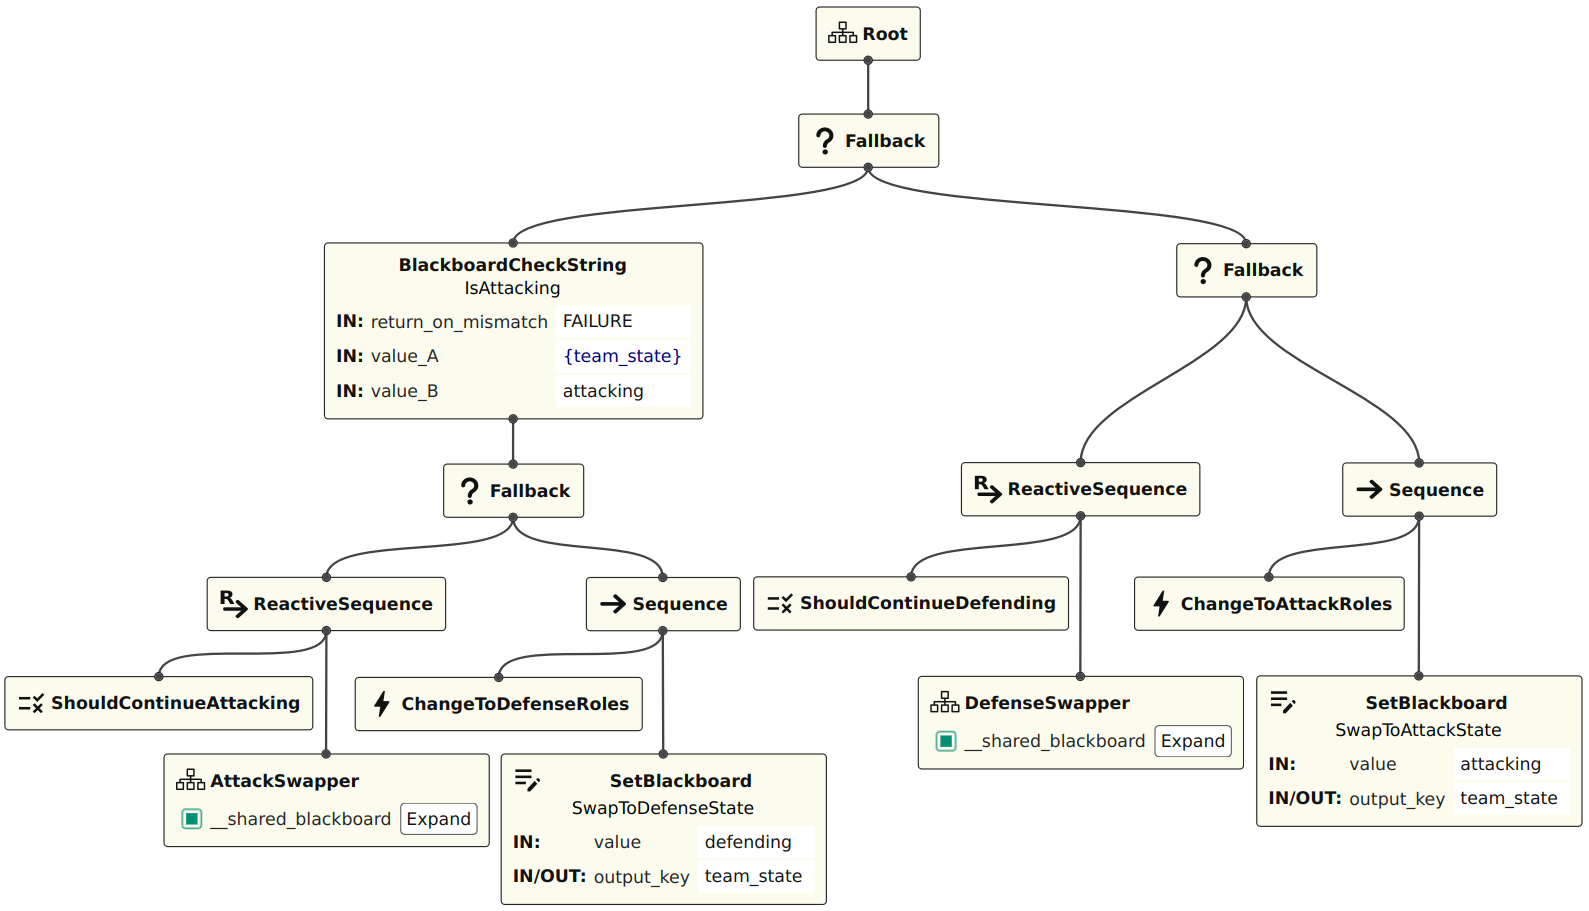
\includegraphics[width=1.0\linewidth]{images/implementation/RolesSwapper.png}
%     \caption{Roles Swapper subtree implementation}
%     \label{fig:roles_swapper_impl}
% \end{figure}

% \subsection{Attack Swapper and Defense Swapper}

% Finally, the \texttt{Attack Swapper} and \texttt{Defense Swapper} subtrees were also implemented taking into account the modifications discussed in Subsection \ref{subsec:common_nodes_impl}, the result is illustrated in Figure \ref{fig:attack_swapper_impl} and \ref{fig:defense_swapper_impl}, respectively.

% Regarding the implementation of the nodes in both of these trees, it is important to note how the nodes that perform the roles changes and swap were developed. To enhance the performance of the trees, these nodes were developed as asynchronous nodes, specifically using coroutines as their foundation. This design choice allows the role changes to be executed in parallel with the rest of the tree, without blocking its execution. The use of coroutines to develop the nodes was possible thanks to the \textit{BehaviorTree.CPP} library, which provides many ways of creating asynchronous nodes.

% \begin{figure}[!h]
%     \centering
%     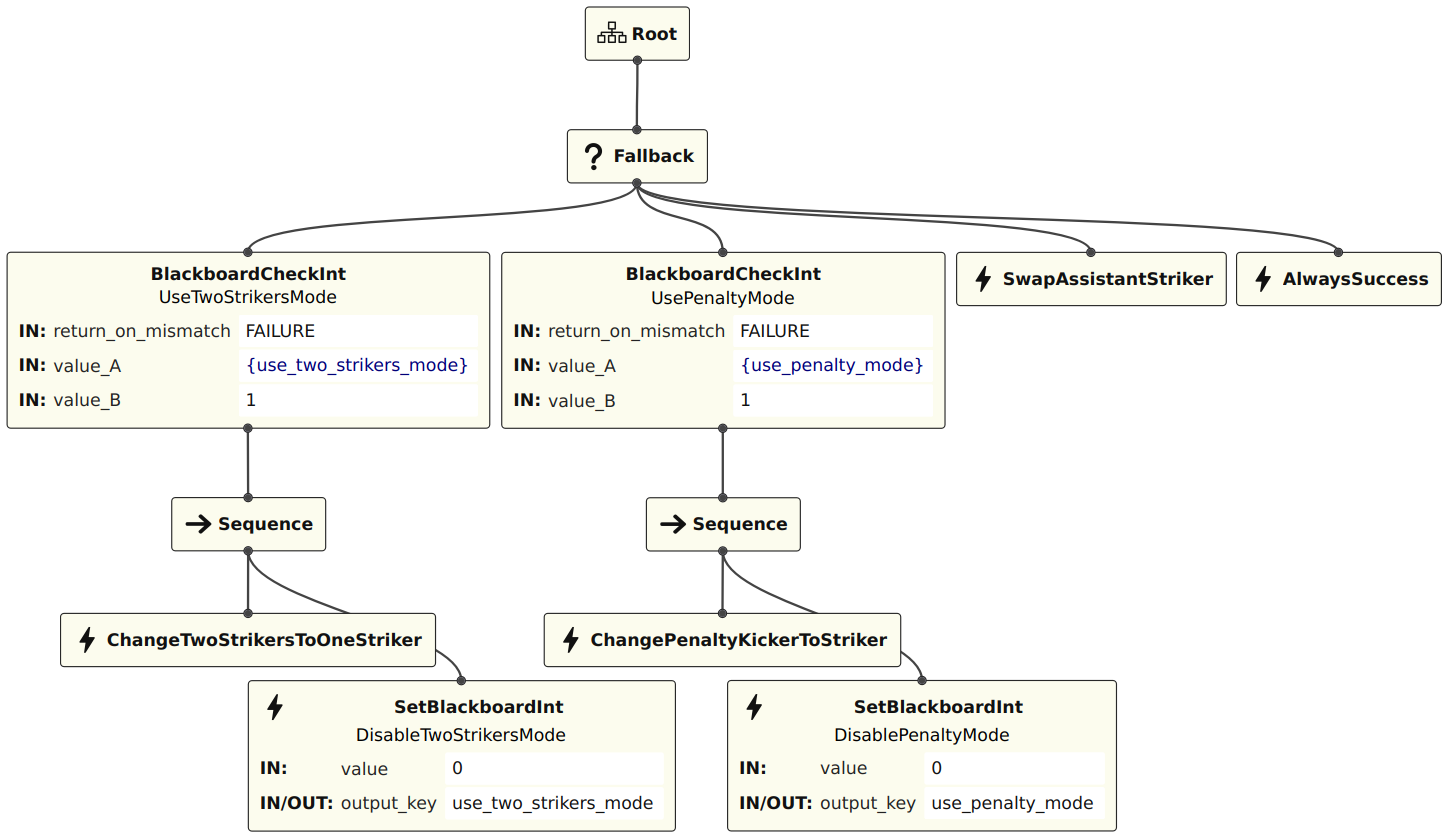
\includegraphics[width=1.0\linewidth]{images/implementation/AttackSwapper.png}
%     \caption{Attack state internal swap subtree implementation}
%     \label{fig:attack_swapper_impl}
% \end{figure}

% \begin{figure}[!h]
%     \centering
%     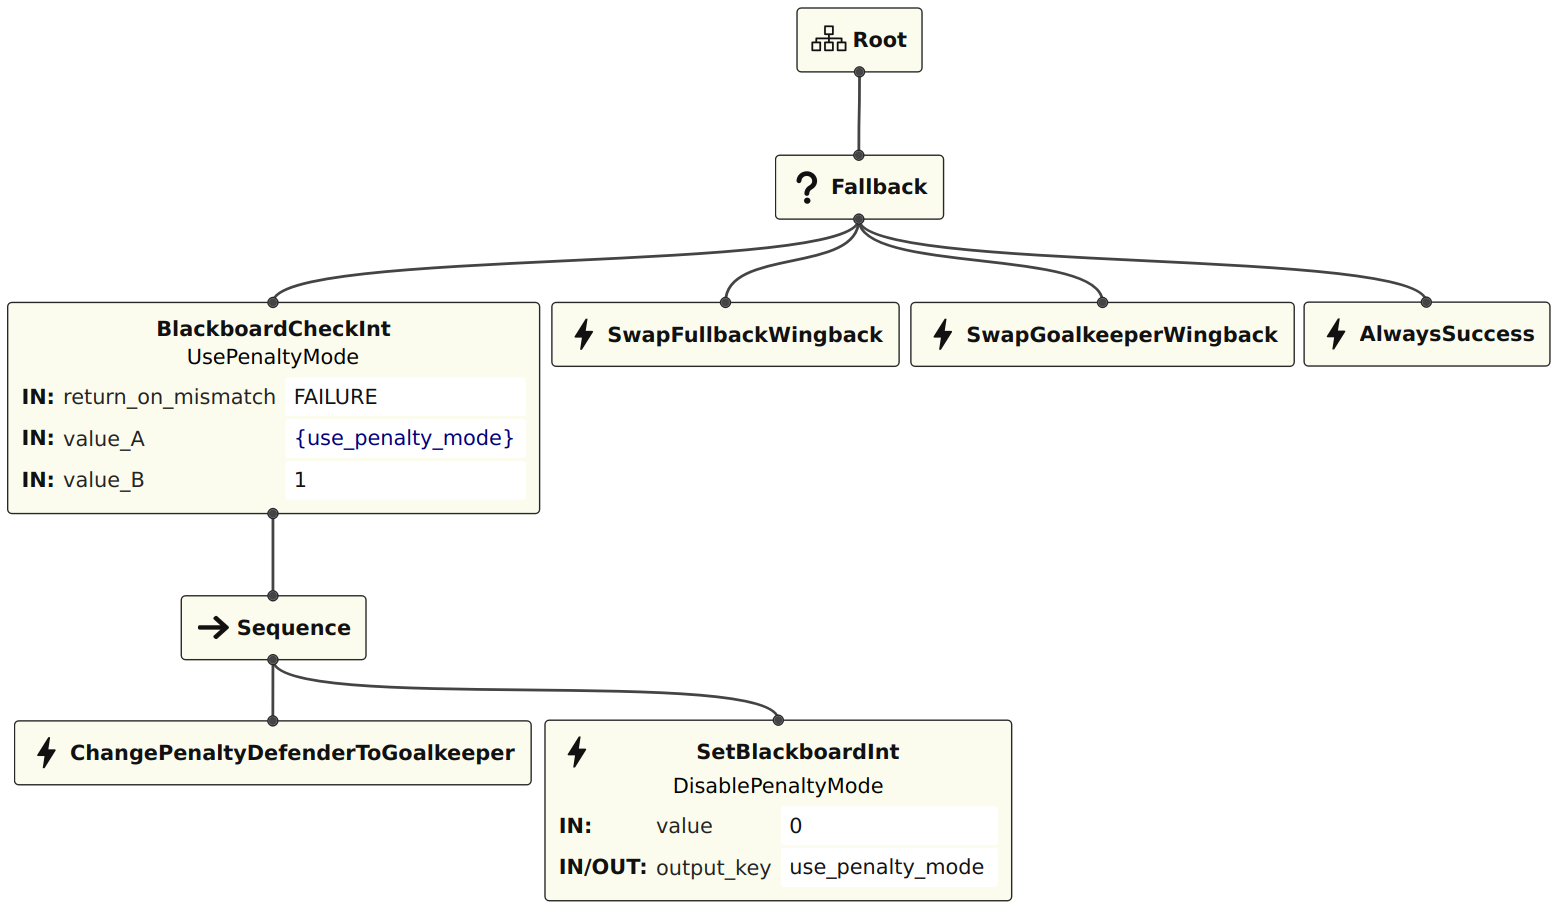
\includegraphics[width=1.0\linewidth]{images/implementation/DefenseSwapper.png}
%     \caption{Defense state internal swap subtree implementation}
%     \label{fig:defense_swapper_impl}
% \end{figure}